\documentclass{article}
\usepackage{booktabs}
\usepackage{geometry}
\usepackage{enumerate}
\usepackage{setspace}
\usepackage{amsthm}
\usepackage{amsmath,amssymb}
\usepackage{amstext}
\usepackage[hidelinks]{hyperref}
\usepackage{graphicx}
\usepackage{setspace}
\usepackage{color}

\geometry{a4paper,scale=0.85}
\linespread{1.5}

\newtheorem{definition}{Definition}[section]
\newtheorem{theorem}{Theorem}[section]
\newtheorem{lemma}{Lemma}[section]
\newtheorem{proposition}{Proposition}[section]
\newtheorem{remark}{Remark}[section]
\newtheorem{corollary}{Corollary}[section]

\def\d{\mathrm{d}}
\def\Cov{\mathrm{Cov}}
\def\E{\mathrm{E}}
\def\Var{\mathrm{Var}}
\def\unf#1{\textcolor{blue}{#1}}

\title{VE401 Project Notes}
\author{ARessegetes Stery}
\date{\today}

\setlength{\parindent}{0pt}

\begin{document}
\maketitle

\begin{spacing}{2}
    \tableofcontents
\end{spacing}

\newpage
\section{Summary of the Testing Rules}

We first summarize all the significant parts of the criterion and explain the choices 

\unf{Unify the terminology: \textbf{batch} for the population, \textbf{package} for individual sample, and \textbf{samples} for the general samples}

\subsection{Valid Interval for sample mean $\overline{q}$}

This is the case for test for sample mean with unknown variance. Then the test statistic with mean of the process $\mu$ is 
$$
T_{n-1} = \dfrac{\overline{X} - \mu}{S/\sqrt{n}}
$$
should follow a $T$-distribution with $n-1$ degrees of freedom. Suppose that the random variable (process) generating all the samples yields a mean of exactly $Q_n$, since a confidence level of 99.5\% is desired, we would like 99.5\% of the times when a sample is generated using the process, it will fall above the threshold. Then, the lower bound of $\overline{q}$ is the lower bound of a 99.5\% confidence interval for the test statistic $T_{n-1}$ when $\mu = Q_n$, which gives
$$
\dfrac{\overline{X} - \mu}{S/\sqrt{n}} \geq -t_{0.995, n-1} \quad\Leftrightarrow\quad \overline{X}\geq\mu-\dfrac{S}{\sqrt{n}}t_{0.995, n-1}
$$ 
which corresponds to $\lambda\cdot s$ in the third column of the table. 

Note that the $t_{0.995}$ in the table actually refers to $t_{0.995, n-1}$; \unf{include comparison figures in the report}

This can be formalized to be a Fisher Test: we set up the null hypothesis to be
$$
H_0: \mu \geq Q_n
$$
and we seek to either not reject it, or reject it at a level of significance less than or equal to 0.5\%. 

\unf{May want to first address the problem of formalizing the experiment into a Fisher Test and then argue on the critical region.}

\subsection{Choice of Sample Size}

First of all, if the total size of shipment is quite small (less than or equal to 10), sampling is not necessary since examining all the individual package is sufficient enough and not costly. 

For other cases, we are trying to make an inference on the proportion of the samples that do not fall short in the amount of product. But instead of having samples generating from a repeatable process, we are taking a portion from the population without replacing it. This causes a perturbation on the resulting sample variance. Therefore, in order to determine the appropriate sample size, we need to first investigate the sample variance in this case. We provide the following theorem:

\begin{theorem}[Sample Variance for Sampling without Replacement]
    Suppose that we draw $n$ samples from a population of size $N$ and variance $\sigma$. Then the sample variance is
    $$
    \Var(\overline{X}) = \dfrac{\sigma^2}{n}\cdot\dfrac{N-n}{N-1}
    $$
\end{theorem}

We refers to [\unf{add reference}] for the proof

\begin{proof}
    Recall how the proof is conducted in the case where $N$ is infinite:
    $$
    \Var[\overline{X}] = \Var\left[\frac{1}{n}\sum\limits_{k=1}^n X_k\right] = \dfrac{1}{n^2} \sum_{1\leq i,j\leq n}\Cov[X_i, X_j]
    $$
    In the case where $N$ is infinite, the influence of replacement is almost zero; and we could conclude that all the $X_i$s are independent, which gives 
    $$
    \Cov[X_i, X_j] = \begin{cases}
        \Var[X_i] &, i = j\\
        0 &, i\neq j 
    \end{cases}
    $$
    But if $N$ is finite, the covariances should be calculated manually. Denote $\xi_i$ to be the values of the samples, $n_i$s the number of samples sharing value $\xi_i$ and $p_i$ the probability of obtaining value $\xi_i$, we have
    \begin{align*}
        \E[X_1 X_2] & = \sum\limits_{i, j}\xi_i \xi_j p_{ij} \\
                    & = \sum\limits_{i}\xi_i p_i \sum\limits_{j} \xi_j \frac{p_{ij}}{p_i} \\
                    & = \sum\limits_{i}\xi_i p_i \left(\sum\limits_{j}\left(\xi_j\frac{N p_j}{N-1}\right) - \frac{\xi_i}{N-1} \right) \\ 
                    & = -\frac{1}{N-1}\underset{\E[X^2]}{\underbrace{\sum\limits_{i}\xi_i^2 p_i}} + \frac{N}{N-1}\left(\sum\limits_{j}\xi_j p_j\right)^2 \\
                    & = -\frac{1}{N-1}\left(\sigma^2 + \mu^2\right) + \frac{N}{N-1}\mu^2 \\
                    & = -\frac{1}{N-1}\sigma^2 + \mu^2
    \end{align*}
    which gives the covariance of two random samples
    $$
    \Cov[X_i, X_j] = \E[X_i X_j] - \E[X_i]\E[X_j] = -\frac{1}{N-1}\sigma^2
    $$
    and the variance of $\overline{X}$:
    $$
    \Var[\overline{X}] = \frac{1}{n}\sigma^2 + \frac{n-1}{n}\Cov[X_i, X_j] = \dfrac{\sigma^2}{n}\cdot\dfrac{N-n}{N-1}
    $$
\end{proof}

Then we can infer the adequate size of sample for inference on proportion given that the population is finite with size $N$. 

\begin{theorem}[Sample Size for Finite Population]
    For a sample retrieved from a population of size $N$, to ensure the margin of error (half of the width of confidence interval) $d$ at confidence level $\alpha/2$ for two-sided test, we need the sample size $n$ to be at most
    \begin{equation}\label{ssfinite}
    n\approx \dfrac{z_{\alpha/2}N}{4d^2(N-1)+z_{\alpha/2}}
    \end{equation}
\end{theorem}

\begin{proof}
    The confidence interval of this estimation for the proportion is given as
    $$
    p = \hat{p}\pm z_{\alpha/2} \sqrt{\hat{p}(1-\hat{p})\cdot \dfrac{N-n}{n(N-1)}} =: \hat{p} \pm d
    $$
    Requiring $d\geq z_{\alpha/2} \sqrt{\hat{p}(1-\hat{p})\cdot \frac{N-n}{n(N-1)}}$ gives
    $$
    n\geq \dfrac{z_{\alpha/2}\hat{p}(1-\hat{p})N}{d^2(N-1)+z_{\alpha/2}\hat{p}(1-\hat{p})} = \dfrac{z_{\alpha/2}N}{\frac{d^2(N-1)}{\hat{p}(1-\hat{p})}+z_{\alpha/2}}
    $$
    where since $\hat{p}(1-\hat{p})\leq\frac{1}{4}$ the right hand side is bounded above by
    $$
    \dfrac{z_{\alpha/2}N}{\frac{d^2(N-1)}{\hat{p}(1-\hat{p})}+z_{\alpha/2}} \leq \dfrac{z_{\alpha/2}N}{4d^2(N-1)+z_{\alpha/2}}
    $$
    which gives the minimal size of samples to ensure margin of error $d$
    $$
    n\geq \dfrac{z_{\alpha/2}N}{4d^2(N-1)+z_{\alpha/2}}
    $$
\end{proof}

The choice of sample size $n$ based on knowledge of population size $N$ is demonstrated in the following table. If the choices of numbers are reasonable, using \eqref{ssfinite} with $z_{\alpha/2} = z_{0.995} = 2.575$ we should see that the estimated $d$ values are consistent. 

\begin{table}[htbp]
    \centering
    \begin{tabular}{ccc}
        \toprule
        $N$ & $n$ & Estimated $d$-value \\
        \midrule
        1-10 & $N$ & N/A \\
        11-50 & 10 & [0.08, 0.23] \\
        51-99 & 13 & [0.19, 0.21] \\
        100-500 & 50 & [0.08, 0.11]\\ 
        501-3200 & 80 & [0.08, 0.09]\\
        $>$3200 & 125 & [0.08, 0.09] \\
        \bottomrule
    \end{tabular}
    \caption{Tabulated Values for Population Size $N$ and Corresponding Sample Size $n$ [\unf{proj material}]}
\end{table}

with which we have the conclusions

\begin{itemize}
    \item The test is organized aiming at tolerance of defective rate for large shipments ($N > 100$) of at most 
    $$
    D = d_{\text{test}} + d_{\text{tolerance}} = 11\% + \frac{5}{80} = 17\%
    $$
    where $d_{\text{test}}$ is the margin of error for the test, which is at most 0.11 for $N > 100$, and $d_{\text{tolerance}}$ is the tolerable defective rate in the samples examined, which is at most $5/80$ for $N\in[501, 3200]$. 
    \item For small shipments $N \leq 100$, the defective rate allowed can be as high as
    $$
    D = d_{\text{test}} + d_{\text{tolerance}} = 21\% + \frac{1}{13} = 29\%
    $$
    with the same notation. Specifically, for $N\in[51, 99]$ the lower bound of largest allowed defective rate is 0.19, which is a relatively high defective rate. This choice of design may result from avoiding separating into too many cases for small $N$ or reasons specific with products with small shipments, or may be just an error in setting up the criterion.
    \item In order to ensure the coherence exhibited in the rules, we suggest that the \textbf{$n$ for $N$ in 51-99 should be changed into 32}, which is solved with $d=0.08$ using \ref{ssfinite}. In following discussions on this table we will comment on the result with calibrated $n$ value separately besides using the originally tabled value. 
\end{itemize}

\subsection{Maximum Allowed Number of $T_1$ shortage}

\subsubsection{Specification of the Requirements}

\begin{definition}[$T_1$ Error, $T_2$ error]
    \unf{ref[2.1.2.3/4]} For a given standard $Q$ with the applicable tolerable deficiency $T$, a sample $Q_i$ is said to be of $T_1$ error if
    $$
    Q-2T \leq Q_i < Q-T
    $$
    and is said to be of $T_2$ error if
    $$
    Q_i < Q-2T
    $$
\end{definition}

We first summarize the criterion for inspection [\unf{5.3}]:

\begin{enumerate}
    \item[(A.1)] The sample mean is no less than the labeled nominal amount.
    \item[(A.2)] The proportion of samples with nominal amount less than the required amount (labeled amount minus the tolerable deficiency) is less than 2.5\%.
    \item[(A.3)] There are no $T_2$ errors in the samples. 
\end{enumerate}

together with the requirement of the inspection\footnote{The sequence of presenting the rules is slightly changed so that they are classified in terms of statistic examined, instead of type of errors.}:
\begin{enumerate}
    \item[(B.1)] If a shipment is correctly manufactured, i.e. with $\mu\geq Q$ where $Q$ is the labeled amount, than the probability of this being rejected is less than 0.5\%.
    \item[(B.2)] If the sample mean is less than $Q-0.74s$, then 90\% of the time we can spot it out (and reject that).
    \item[(B.3)] If the proportion of $T_1$ error is no more than 2.5\%, then the probability of it being rejected is no more than 5\%.
    \item[(B.4)] If the proportion of $T_1$ and $T_2$ error combined is 9\%, then 90\% of the time we can spot it out (and reject that).
\end{enumerate}

Note that the general criterion does not specify the number of $T_1$ errors allowed in the inspection. This depends on the actual size of shipment and needs to be determined accordingly. We now seek to verify the correctness of the tolerable $T_1$ errors in the form. 

In the following discussion, we denote $N_1, N_2$ to be the number of sampled packages of $T_1$ error and $T_2$ error in the population, with $n_1, n_2$ the corresponding number of sampled packages in the samples. The goal is to find the maximum tolerable numbers of $T_1$ error in the samples $k_{N}$ given the size of the whole batch $N$. 

Some of the discussion results are referred from [\unf{international recommendation}].

\subsubsection{Requirement of (B.3)}

If a sample is not rejected according to the criterion, it must satisfy that $P[Q_i < Q - T] \leq 0.025$, i.e. 
$$
\dfrac{Q_i - Q}{T/z_{0.025}} = \dfrac{Q_i - Q}{T/1.96}\sim N(0,1)
$$
Therefore, we require that
\begin{equation}\label{b3}
    P[n_1\leq k, n_2 = 0\mid N_1 = 0.025N, N_2 = 0] \geq 0.95
\end{equation}

\subsubsection{Requirement of (B.4)}

Suppose that 9\% of the batch evaluates to be less than $T$, the distribution of $Q$ evaluates to be
$$
\dfrac{Q_i - Q}{T/z_{0.09}} = \dfrac{Q_i - Q}{T/1.34}\sim N(0,1)
$$
Then 
$$
N_2 = P[\dfrac{Q_i - Q}{T/1.34} < -2.68] = P[Z < -2.68] = 0.0037N, \quad N_1 = [-2.68\leq Z < 1.34] = 0.0863N
$$
The requirement becomes
\begin{equation}\label{b4}
    P[n_1\leq k, n_2 = 0\mid N_1 = 0.0863N, N_2 = 0.0037N] < 0.1
\end{equation}

\subsubsection{Verification of Tolerable $T_1$ Errors}

Since $n_1$ and $n_2$ are chosen simultaneously, they follow a bi-variate hyper-geometric distribution, which has the probability density function
$$
f(n_1, n_2) = \dfrac{\binom{N_1}{n_1}\binom{N_2}{n_2}\binom{N-N_1-N_2}{n-n_1-n_2}}{\binom{N}{n}}
$$
Taking into account of both \ref{b3} and \ref{b4}, we need the stricter restriction on $k$, i.e. the smaller one between the two smallest $k$s that satisfy \ref{b3} and \ref{b4}. We run a numerical program\footnote{Source code is attached as supplementary materials} to evaluate the $k$s. 

The results we obtain are in the \texttt{t1\_en.csv}, \texttt{t1\_wrongdata.csv}, \texttt{t1\_cn.csv} files tested on the case for \unf{p18, International Recom}, raw data in the Chinese guide \unf{4.3.2} and the calibrated data respectively. We conclude that 

\begin{itemize}
    \item Generally the tabled $k$s in the English version \unf{ref} appropriately satisfies the requirement (B.3) and (B.4) 
    \item The $k$ value in the Chinese version of the table are higher than the bound calculated. This results from the smaller $n$ value chosen, making the bound stricter.
    \item We have further evidence that the criterion $n=13$ in the third row of \unf{ref} is indeed a problem as it leads to $k = 0$ in the calculation.
\end{itemize}

\section{Non-Central $T$-Distribution}

If the null hypothesis with a test statistic that follows student T-distribution is false, then non-central student T-distribution shall be used instead as the test statistic for the alternative hypothesis. The random variable
$$
T_{\gamma, \delta}=\frac{Z+\delta}{\sqrt{\chi_\gamma^2/\gamma}}
$$
is said to follow non-central student T-distribution with parameters $\gamma$ degrees of freedom and $\delta$ non-centrality. $\chi_{\gamma}^2$ is Chi-square distributed random variable with $\gamma$ degrees of freedom. Since $\frac{(n-1)S^2}{\sigma^2}$ follows Chi-square distribution with $n-1$ degrees of freedom, so
$$
T_{n-1,\mu\sqrt{n}/\sigma}=\frac{\frac{\Bar{X}-\mu}{\sigma/\sqrt{n}}+\frac{\mu}{\sigma/\sqrt{n}}}{\sqrt{\frac{(n-1)S^2}{\sigma^2}\frac{1}{n-1}}}=\frac{\Bar{X}}{S/\sqrt{n}}
$$
is non-central student T-distributed with $n-1$ degrees of freedom and $\frac{\mu\sqrt{n}}{\sigma}$ non-centrality.

We first set up the null hypothesis and the alternative hypothesis. Under the context of the test, we would want the hypotheses to be
$$
H_0 : \mu\geq\mu_0 \quad\quad\quad\quad H_1 : \mu\leq\mu_0 - \sigma
$$
where we hope not to reject $H_0$ if the sample is obtained in the worst case allowed, i.e. from a batch with mean $\mu_0$. The probability of conducting a Type I Error, which is that of rejecting samples from the boundary case of tolerable production, is designated to be $\alpha = 0.005$. This gives the critical region
$$
\text{We reject }H_0\text{ if the statistic } \dfrac{Z}{\sqrt{\chi_{\gamma}^2/\gamma}} \text{ falls in}\ \left(-\infty, -t_{0.005, n-1}\right]
$$
and an approach to calculate the probability of conducting a Type II Error ($\beta$)
$$
\beta = \int_{-t_{0.005, n-1}}^{\infty} f_{T_{n-1, \frac{\mu\sqrt{n}}{\sigma}}}(x) \d x
$$
This gives the Operating Characteristic (OC) Curve as below:

\begin{figure}[htbp]
    \centering
    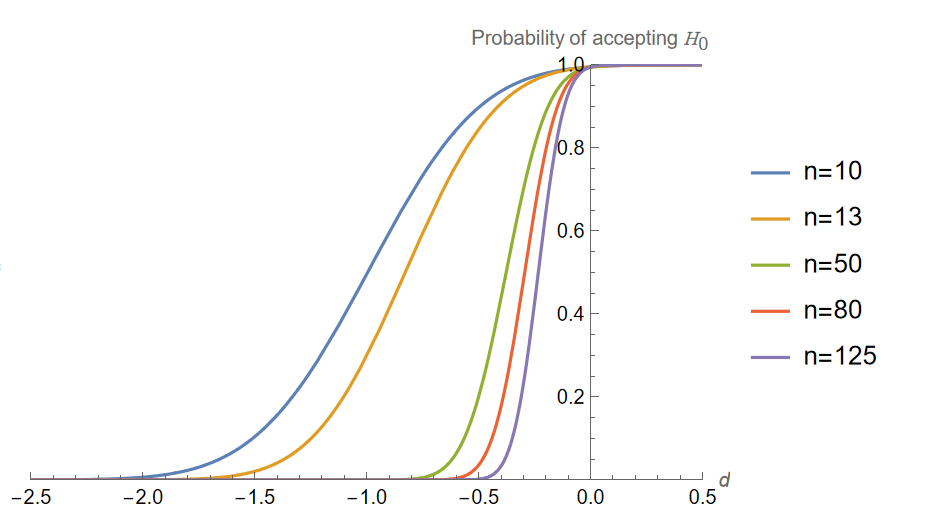
\includegraphics[scale=0.5]{img/oc_noncentral_t.png}
    \caption{OC Curve for One-Tailed Test of Noncentral $T$-Distribution with $n$ Specified in Table 4.3.2}
\end{figure}

From the OC Curve we can see that the test is fairly powerful. With a sample size of $n\geq50$ we can ensure that for samples with average of shortfall at least one standard deviation in package contents, we will almost surely reject $H_0$.

Quantitatively, calculating the results explicitly gives

\begin{table}[htbp]
    \centering
    \begin{tabular}{cc}
        \toprule
        $n$ & $P[\text{Reject }H_0]$  \\
        \midrule
        10 & 50.4\% \\
        13 & 70.1\% \\
        50 & 99.9\%  \\
        80 & 100\% \\ 
        125 & 100\% \\
        \bottomrule
    \end{tabular}
    \caption{Probability of Rejecting $H_0$ for Batches not Fulfilling Requirements}
\end{table}


\end{document}